%
% Sección de algoritmos tokenizadores.
% Artículo.
% Proyecto Lovelace.
%

\section{Algoritmos tokenizadores}

Como el enfoque de este artículo es ver a la tokenización como un servicio
(figura \ref{figura:arquitectura_tokenizacion}), la interfaz para los procesos
de tokenización y detokenización, desde el punto de vista de los usuarios del
servicio, es sumamente simple: el proceso de tokenización es una función $ E:
\mathcal{X} \rightarrow \mathcal{Y} $ y el de detokenización es  simplemente la
función inversa $ D: \mathcal{Y} \rightarrow \mathcal{X} $, en donde $
\mathcal{X} $ y $ \mathcal{Y} $ son los espacios de números de tarjetas y
tokens, respectivamente. Ambos conjuntos son cadenas de dígitos de entre 12 y 19
caracteres. Los números de tarjeta cuentan con un dígito verificador que hace
que \texttt{algoritmoDeLuhn(X) = 0}; los tokens cuentan con un dígito
verificador que hace que \texttt{algoritmoDeLuhn(Y) = 1}. El último punto es con
el propósito de que sea posible distinguir entre un número de tarjeta y un token.

El PCI SSC (\textit{Payment Card Industry Security Standard Council}) establece
en sus guías de tokenización la siguiente clasificación para los algoritmos
tokenizadores~\cite{pci_tokens}:

\begin{figure}
  \begin{center}
    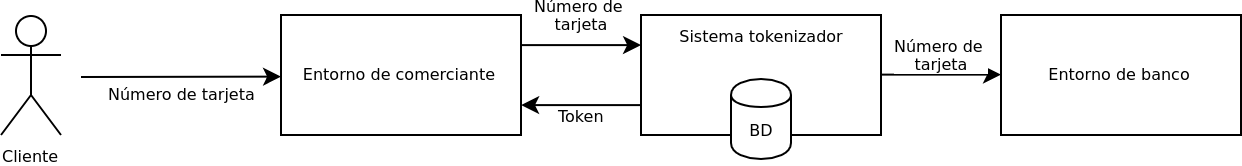
\includegraphics[width=1.0\linewidth]{diagramas/sistema_tokenizador.png}
    \caption{Arquitectura típica de un sistema tokenizador.}
    \label{figura:arquitectura_tokenizacion}
  \end{center}
\end{figure}

\begin{itemize}
  \item Métodos reversibles. Aquellos para los cuales es posible regresar al
    número de tarjeta a partir del token.
    \begin{itemize}
      \item Criptográficos. Ocupan un esquema de cifrado simétrico: el número
        de tarjeta y una llave entran al mecanismo de tokenización para obtener
        un token; el token y la misma llave entran al mecanismo de
        detokenización para obtener el número de tarjeta original.
      \item No criptográficos. Ocupan una base de datos para guardar las
        relaciones entre números de tarjetas y tokens; el proceso de
        detokenización simplemente es una consulta a a la base de datos.
    \end{itemize}
  \item Métodos irreversibles. Aquellos en los que no es posible regresar al
    número de tarjeta original a partir del token.
    \begin{itemize}
      \item Autenticable. Permiten validar cuando un token dado corresponde a
        un número de tarjeta dado.
      \item No autenticable. No permiten hacer la validación anterior.
    \end{itemize}
\end{itemize}

% TODO: mejorar crítica a segunda categoría.

La denominación \textit{no criptográficos} resulta totalmente confusa, pues en
realidad todos los métodos conocidos que caen en las categorías de arriba ocupan
primitivas criptográficas. La segunda categoría (los irreversibles) carece de
utilidad para aplicaciones que procesan pagos con tarjetas de crédito, pues la
habilidad de regresar al número de tarjeta a partir de su token es uno de los
requerimientos principales para los sistemas tokenizadores. Por lo anterior, en
este trabajo se propone una clasificación distinta:

\begin{itemize}
  \item Métodos criptográficos. Todos aquellos que ocupan herramientas
    critográficas para operar.
    \begin{itemize}
      \item Reversibles. Ocupan un esquema de cifrado simétrico: el número
        de tarjeta y una llave entran al mecanismo de tokenización para obtener
        un token; el token y la misma llave entran al mecanismo de
        detokenización para obtener el número de tarjeta original. El término
        \textit{reversible} es porque se puede regresar al número de tarjeta sin
        ayuda de herramientas externas, como una base de datos.
      \item Irreversibles. Ocupan herramientas criptográficas para generar el
        token de un número de tarjeta. Operan como funciones de un solo sentido:
        la única manera de regresar al número de tarjeta a partir de un token es
        mediante un ataque por fuerza bruta o mediante herramientas externas,
        como una base de datos.
    \end{itemize}
  \item Métodos no criptográficos. Aquellos posibles métodos que no ocupen
    herramientas relacionadas con la criptografía; por ejemplo, un generador de
    números realmente aleatorio (TRNG, \textit{True Random Number Generator}).
\end{itemize}

La clasificación de los \textit{no criptográficos} solamente se propone para
abarcar métodos de los cuales realmente se pueda decir que no se relacionan con
la criptografía. En este trabajo no se presenta ningún método que clasifique en
esa categoría.

A continuación se presentan algunos de los algoritmos tokenizadores más comunes.
Al final de cada sección se explica en qué categoría cae según las dos
clasificaciones anteriores.

\subimport{/}{tkr}
\subimport{/}{ffx}
\subimport{/}{bps}
\subimport{/}{drbg}
